\documentclass[fontsize = 14pt, paper= a4]{jlreq}

\usepackage{graphicx}
\usepackage{color}
\begin{document}

\title{プログラミング 第一回 レポート}
\author{202212022 田島瑞起}
\date{2023/05/17}
\maketitle

\section{はじめに}
今回の課題では
、
\begin{enumerate}
\item Linux のファイル操作コマンドを表形式でまとめる。
\item C 言語プログラムを図(テキスト形式)として掲載する
\item Linux コマンドを操作しているところを図として掲載する
\item 本の紹介をする 以上4 点の設問に対しLaTeX を用いて解答する。
\end{enumerate}

以上四点の設問を満たすpdf ファイルをLaTeX を用いて作成する。

\section{Linux操作コマンドについてまとめる}
\subsection{課題内容の説明}
課題内容はこの講義で取り扱ったファイル操作に関するコマンドを表形式で纏めることである。
具体的な要件として、下記五つを満たす必要がある。
\begin{enumerate}
\item 操作オプションの異なるものは別の行として考える
\item 一行はコマンド名、コマンド例、説明を列とする
\item 7~12行の範囲に収まるようにコマンドを選ぶ
\item 節の中には、本文を記述して、表番号を参照するようにすること
\item PDF化する際、表がページからはみ出ないように調節すること
\end{enumerate}

\subsection{課題への取り組み方針}
Linuxコマンドにて最も重要であるディレクトリ操作一般について纏める。
\subsection{解答結果}

\begin{table}[h]
  \centering
  \caption{Linuxコマンド}
  \label{tab:linux_cmd_list}
  \begin{tabular}{|p{30mm}|p{30mm}|p{80mm}|} \hline
    
    コマンド名 & コマンド例 & コマンド説明 \\  \hline
    
    ls&ls&カレントディレクトリ配下を表示 \\  \hline

    ls -a & ls -a & 隠しファイル含めすべてを表示する \\ \hline

    pwd & pwd & 現在のパスを表示する \\ \hline

    cd 元1 & cd test & 対象ディレクトリに移動する \\ \hline

    cd ../ & cd ../ & 親ディレクトリに移動する \\ \hline

    mkdir 元1 & mkdir test & 対象ディレクトリを作成 \\ \hline

    rm 元1 & rm test.tex & 対象ファイルを削除する \\ \hline

    rmdir 元1 & rmdir test & 対象ディレクトリを削除する \\ \hline
  \end{tabular}
  
\end{table}
\subsection{解答結果に対する説明}
table環境を使用して表を作成し,題意を満たすように列幅を変更して文字がはみ出ないように調節した。(表\ref{tab:linux_cmd_list})
\subsection{考察}
(表\ref{tab:linux_cmd_list})は上述された5つの要件を満たしている。
表は一行ごとに色が変わると見やすいと感じたので次回以降実装する。

\section{プログラムを図として掲示せよ}
\subsection{課題内容の説明}
C言語のソースプログラムを図として挿入しPDF化する。
PDF化する際に下記要件を満たす必要がある。
\begin{enumerate}
\item プログラムの各行に番号をつけること
\item プログラムの各文字をテキストとしてあるかえること
\item プログラム部分はタイプライタ体で表示されること
\item 本文を作成して図を参照すること
\item PDF化した際にページをはみ出ないこと
\end{enumerate}

\subsection{課題への取り組み方針}
cat -n コマンドを用いてソースコードに行番号を付与した後に,そのテキストを、verbatim環境を用いてそのまま埋め込む。
\subsection{解答結果}

\begin{verbatim}
     1       1  #include <stdio.h>
     2       2
     3       3  void sort(int n, int num[]){
     4       4    int i, j;
     5       5
     6       6    for(i=0; i<n-1; i++){
     7       7      for(j=i+1; j<n; j++){
     8       8        if (num[i] > num[j]){
     9       9          int tmp;
    10      10          tmp = num[i];
    11      11          num[i] = num[j];
    12      12          num[j] = tmp;
    13      13        }
    14      14      }
    15      15    }
    16      16  }
    17      17
    18      18  int main(int ac, char* av[]){
    19      19    int num[] = { 3, 1, 4, 5, 9, 2, 6, 8, 7 };
    20      20    int i;
    21      21
    22      22    for(i = 0; i < 9; i++){
    23      23      printf("%3d", num[i]);
    24      24    }
    25      25    printf("\n");
    26      26
    27      27    sort(9, num);
    28      28
    29      29    for(i = 0; i < 9; i++){
    30      30      printf("%3d", num[i]);
    31      31    }
    32      32    printf("\n");
    33      33  }


\end{verbatim}

\subsection{解答結果に対する説明}

課題の取り組み方針にて書いたとおりに実行した

\subsection{考察}

ソースコード表は、上述した要件5つを満たしている。
ソースコードも行ごとに色が変化すると見やすいと感じた。

\section{Linux操作中の画面を図として挿入する}

\subsection{課題内容の説明}
全額計算機システムのLINUX環境を使用しているところをキャプチャして、図として挿入する。
今課題は下記要件を満たす必要がある。

\begin{enumerate}
\item 何をしているところなのか説明を入れること
\item どのキャプチャ方法を用いたのか示すこと
\item そのキャプチャ方法の操作方法を説明として含めること
\item 図をLatexの機能で参照すること
\item PDF化した際にページをはみ出ないこと
\end{enumerate}

\subsection{課題の取り組み方針}
今回はWindowsPcを用いてスクリーンショットを取り、それをfigure環境にて埋め込む。
\subsection{解答結果}

\begin{figure}[htbp]
  \centering
  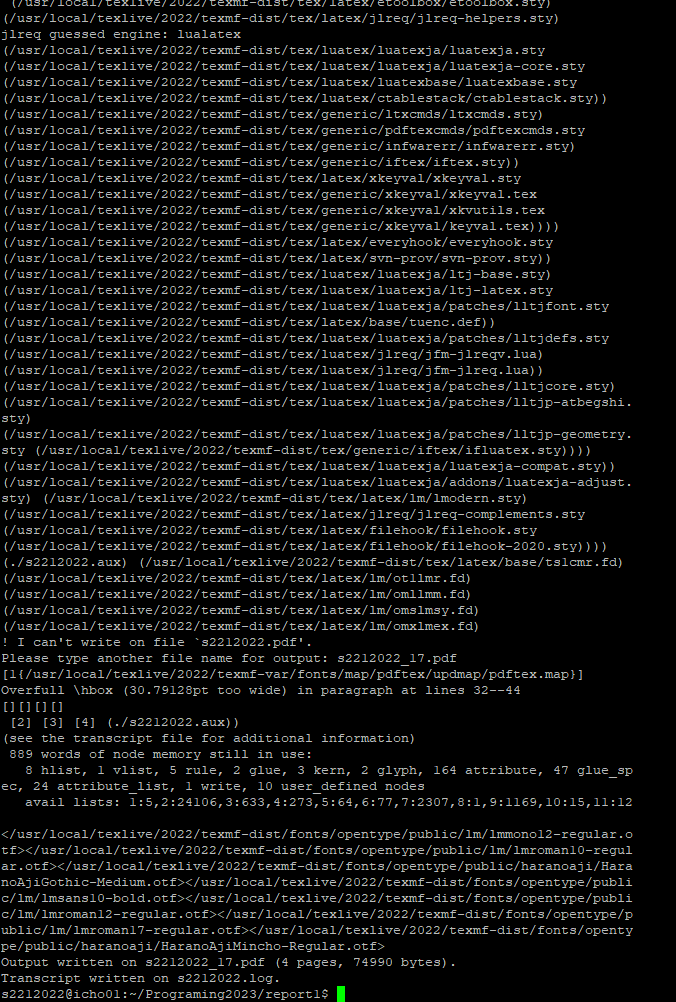
\includegraphics[width=100mm]{linux.png}
  \caption{linuxを操作している画面}
  \label{fig:linux_using}
\end{figure}

\subsection{解答に対しての説明}
\ref{fig:linux_using}を取り組み方針の通り解答した
\subsection{考察}
解答は上述した要件を満たしている。

\section{本の紹介}
\subsection{課題内容}
今課題では本の紹介をする。
下記要件を満たす必要がある。
\begin{enumerate}
\item 本を三冊紹介する
\item そのタイトルの後ろに文献番号を参照する
\item BiBTeXを用いて文献情報を明示すること
\end{enumerate}

\subsection{課題の取り組み方針}
好きな国内哲学者二人と、フーコーについて簡単に取り上げる。

\subsection{解答結果}

現代思想入門\cite{chiba}は現代思想というポストモダン思想について書かれた入門書であり、新書ということもあってか幅広くの人に読まれている。
ポストモダン思想というのは、その思想自体を揶揄するようなワードとして一部使用されているが、簡単に要約すれば、白黒物事を決めたときに零れ落ちてしまうリアリティーについて取り扱う学問体系のことを指す。
千葉はこの著作の中で入門書を読み終えた後にぜひ読んでほしいという本を2つ紹介している。一つ目が「ジャックデリダについて」\cite{azuma}である。この本はポストモダン思想家の中でも特別に重要なデリダについて、紹介した本である。デリダは際について着目した人間で、私たちが以下に二項対立から逃れられず、またそれが無意味であるということを鮮やかに導いた。次に紹介されているのが、「監獄の誕生」\cite{foo-koo}である。フーコーは現在直面している私達の問題が歴史的に構成されているという事実を鮮やかに書き出した人物であり、この「監獄の誕生」では精神病者が監獄というモデルから生み出された産物であるという一見関連しないような対象の関係性を見事に見抜いた。以上3つの本は現代思想を国内で学ぼうとした時に有用な書であるから、是非を読んでほしい。

\subsection{解答結果に対する説明}
bibファイルを生成して,bibtexコマンドを用いて、bblファイルを生成したのちに、本文中に番号付きで文献参照を行った。
\subsection{考察}
上述した要件を満たしている。
文献参照は実装に必要なコマンドの順番を間違えるとエラーが起こり、またlualatexコマンドも二回打たないと実装できない点が面倒だった。
\section{課題全体の感想}
一回texファイルをまとめて削除したことにより鬱状態に陥ったが、二回分演習したおかげで、何も見ずにlatexを使いこなせるようになってよかった。
重要なファイルは小まめに保存して、コピーを作成することの重要性に気が付いた。

\bibliographystyle{plain}
\bibliography{s2212022}
\end{document}
